\documentclass[12pt,letterpaper,noanswers]{exam}
\usepackage[usenames,dvipsnames,svgnames,table]{xcolor}
\usepackage[margin=0.9in]{geometry}
\renewcommand{\familydefault}{\sfdefault}
\usepackage{multicol}
\usepackage{wrapfig}
\pagestyle{head}
\definecolor{c03}{HTML}{FFDDDD}
\header{AM 22b Class 06}{}{Feb 08: cross-product and determinant}
\runningheadrule
\headrule
\usepackage{graphicx} % more modern
\usepackage{amsmath} 
\usepackage{amssymb} 
\usepackage{hyperref}
\usepackage{tcolorbox}

\usepackage[numbered,autolinebreaks,useliterate]{mcode}

\newcommand{\mb}[1]{\underline{#1}}

\begin{document}
 \pdfpageheight 11in 
  \pdfpagewidth 8.5in




% I need to review the torus trajectories...

\begin{itemize}
% \item There is a pre-class assignment (20 minutes of videos + a few WeBWorK exercises) due at 10am this Monday.  It is available on Canvas.
\itemsep0em
    \item There is a skill check today, and an optional retake for skills C02 and C03 (do one, both, or none).
    \item The next skill check will be this Friday (skills C06 and C07).
    \item PSet 02 is due on Thursday Feb 11th at 6pm.
\end{itemize}

\hrule
\vspace{0.2cm}



\noindent\textbf{Big picture}

Today we are spending a little more time on vector products.  Determinants provide a convenient notation for the scalar triple product and for the cross product.  We will work with that notation today.  These vector products will become very important in March: we'll be using them all of the time once we start working with functions that have vectors for their output.

\vspace{0.2cm}
\hrule
\vspace{0.2cm}

\noindent\textbf{Skill Check C06 Practice}

\begin{questions}
\item Compute the scalar triple product of $\mb{u} = \left(\begin{array}{c}1 \\ 3\\ 2\end{array}\right)$, $\mb{v} =\left(\begin{array}{c}0 \\ -1\\ 1\end{array}\right)$, $\mb{w}=\left(\begin{array}{c} 2 \\ 1\\ 0\end{array}\right)$ using a determinant.

\framebox(150,30){ scalar triple product: \hfill }
\end{questions}

\vspace{0.2cm}

\hrule
\vspace{0.2cm}

\noindent\textbf{Skill Check C06 solution}
\begin{questions}
\item We can compute either $\text{det}\left([\mb{u}\ \mb{v}\ \mb{w} ]\right)$ or $\text{det}\left(\left[\begin{array}{c}\mb{u}^T \\ \mb{v}^T \\ \mb{w}^T \end{array}\right]\right)$ (they will be equal).


I'll expand using the top row, so $+,-,+$.

\begin{align*}
    \text{det}\left(\begin{array}{c c c}1 & 3 & 2 \\ 0 & -1 & 1 \\ 2 & 1 & 0 \end{array}\right) &= (1) \left\vert \begin{array}{c c} -1 & 1 \\ 1 & 0\end{array}\right\vert- (3) \left\vert \begin{array}{c c} 0 & 1 \\ 2 & 0\end{array} \right\vert + (2) \left\vert \begin{array}{c c}0 & -1 \\ 2 & 1\end{array} \right\vert \\
    &= (1)(0-1) -3(0-2) +2(0+2) \\
    &= -1 +6 + 4\\
    &= 9.
\end{align*}

If I choose the middle row, I need to use $-,+,-$ rather than $+,-,+$:
\begin{align*}
\text{det}\left(\begin{array}{c c c}1 & 3 & 2 \\ 0 & -1 & 1 \\ 2 & 1 & 0 \end{array}\right) &= -(0) + (-1) \left\vert \begin{array}{c c} 1 & 2 \\ 2 & 0\end{array} \right\vert - (1) \left\vert \begin{array}{c c}1 & 3 \\ 2 & 1\end{array} \right\vert \\
    &=  -(0-4) -(1-6) \\
    &= 4 +5\\
    &= 9.
\end{align*}
Check in Matlab:
\begin{lstlisting}
det([1 3 2; 0 -1 1; 2 1 0])
\end{lstlisting}
\end{questions}

\vspace{0.2cm}
\hrule
\vspace{0.2cm}


\noindent\textbf{Matlab code example 1}
\begin{lstlisting}
%% Plot a surface
f1 = @(x,y) x.^2+y.^2;
syms x y
figure(1)
subplot(1,3,1)
fsurf(x,y,f1(x,y),[-2 2 -2 2],'edgecolor','none','facecolor','interp')
%% Approximate the surface with parallelograms: show the x=vectors
delt = 0.5;
xcorners = -2:delt:(2-delt);
ycorners = xcorners;
[x1,y1] = meshgrid(xcorners,ycorners);  % bottom left corners.
% turn these into lists:
xlist = x1(:);
ylist = y1(:);
zval = f1(xlist,ylist);
subplot(1,3,2)
% vectors side x
deltx1 = delt + 0*xlist;
delty1 = 0*deltx1;
deltz1 = f1(xlist+deltx1,ylist+delty1)-f1(xlist,ylist);
% plot the vectors.
% quiver3(x,y,z,u,v,w,0) 0 sets the vectors to be actual size (not scaled).
quiver3(xlist,ylist,zval,deltx1,delty1,deltz1,0,'g')
%% Approximate the surface with parallelograms: show the y=vectors
% vectors side y
deltx2 = 0*xlist;
delty2 = delt+0*deltx2;
deltz2 = f1(xlist+deltx2,ylist+delty2)-f1(xlist,ylist);
hold on
quiver3(xlist,ylist,zval,deltx2,delty2,deltz2,0,'m')
%% Find the "area vectors" and plot those
subplot(1,3,3)
hold off
quiver3(xlist,ylist,zval,deltx1,delty1,deltz1,0,'g')
hold on
quiver3(xlist,ylist,zval,deltx2,delty2,deltz2,0,'m')
crossvecs = cross([deltx2,delty2,deltz2],[deltx1,delty1,deltz1]);
quiver3(xlist,ylist,zval,crossvecs(:,1),crossvecs(:,2),crossvecs(:,3),0,'k')
%% format plots
for plotnum = 1:3
    subplot(1,3,plotnum)
    axis equal
    axis([-3 3 -3 3 -0.5 8])
    xlabel('x'); ylabel('y'); zlabel('z')
end
\end{lstlisting}


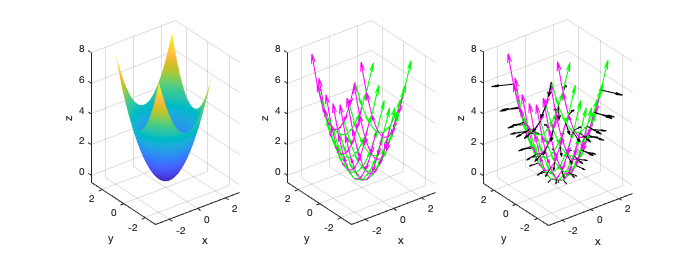
\includegraphics[width=0.7\textwidth]{img/C05wireframe.png}



\vspace{0.2cm}
\hrule
\vspace{0.2cm}




\noindent\textbf{Teams}

Same groups as last time: your icebreaker today is to talk a little about what classes you are taking with your team.
\begin{multicols}{2}

1.  student names

\end{multicols}

%\vspace{0.2cm}
\hrule
\vspace{0.2cm}


\noindent\textbf{Question}.

Figure 13.44 shows the tetrahedron determined by three vectors $\mb{a}, \mb{b}, \mb{c}$.

\begin{tcolorbox}
The \textbf{area vector} of a face is a vector perpendicular to the face, pointing outward, whose magnitude is the area of the face. 
\end{tcolorbox}

We want to show that the sum of the four outward pointing area vectors of the faces equals the zero vector.  

\noindent Discuss how to approach this problem.

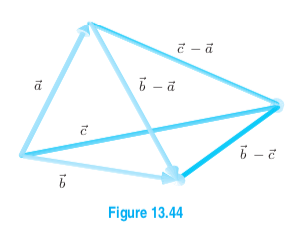
\includegraphics[scale=0.4]{img/C05tetrahedron.png}

\vspace{1in}

\vspace{0.2cm}
\hrule
\vspace{0.2cm}

\eject
\noindent\textbf{A little about determinants} \S Appendix E
\begin{tcolorbox}
The \textbf{determinant} of a 2x2 matrix, $A = \left(\begin{array}{c c} a & b \\ c & d \end{array}\right)$, denoted $\text{det} A$, $\left\vert A\right\vert$, or $\left\vert\begin{array}{c c} a & b \\ c & d \end{array}\right\vert$, is given by $\left\vert\begin{array}{c c} a & b \\ c & d \end{array}\right\vert = ad - bc$.

The determinant of a 2x2 matrix $A = \left[\mb{u}\ \mb{v} \right]$ gives the signed \textbf{area of a parallelogram} with sides $\mb{u}$ and $\mb{v}$.  Use the absolute value of the determinant for the area.

The \textbf{determinant is equal to the product of the eigenvalues} of the matrix: For a matrix $A$ with eigenvalues $\lambda_1, \lambda_2,...,\lambda_n$, $\text{det}A = \lambda_1\lambda_2...\lambda_n.$

The \textbf{determinant is equal to the determinant of the transpose}: $\text{det}(A) = \text{det}A^T$.
\end{tcolorbox}

\noindent\textbf{Examples}
\begin{enumerate}
    \item 
Let $A = \left[\begin{array}{c c}0 & 4 \\ 2 & 2 \end{array}\right]$. $A$ has eigenvectors $\left(\begin{array}{c} 1 \\ 1\end{array}\right)$ and $\left(\begin{array}{c} -2 \\ 1\end{array}\right)$. Identify the eigenvalues of $A$.
\vspace{1.2in}

\item Use the eigenvalues to find $\text{det}(A)$.
\vspace{0.2in}

\item Compute $\text{det}(A)$ using the formula for the determinant of a 2 by 2 matrix.
\vspace{0.2in}

\item Sketch the associated parallelogram.
\vspace{1in}

\end{enumerate}

Check in Matlab:
\begin{lstlisting}
eig([0 4; 2 2])
det([0 4; 2 2])
\end{lstlisting}

\begin{tcolorbox}
The \textbf{determinant} of a 3x3 matrix, $A = \left(\begin{array}{c c c} a_1 & a_2 & a_3 \\ b_1 & b_2 & b_3 \\ c_1 & c_2 & c_3 \end{array}\right)$, denoted $\text{det}A$, $\left\vert\begin{array}{c c c} a_1 & a_2 & a_3 \\ b_1 & b_2 & b_3 \\ c_1 & c_2 & c_3 \end{array}\right\vert$, or $\left\vert A\right\vert$, is given by 
\begin{align*}
\text{det}\left[\begin{array}{c c c} a_1 & a_2 & a_3 \\ b_1 & b_2 & b_3 \\ c_1 & c_2 & c_3 \end{array}\right] &= a_1\text{det}\left[\begin{array}{c c c} \square & \square & \square \\ \square & b_2 & b_3 \\ \square & c_2 & c_3 \end{array}\right]-a_2\text{det}\left[\begin{array}{c c c} \square & \square & \square \\ b_1 & \square & b_3 \\ c_1 & \square & c_3 \end{array}\right]+a_3\text{det}\left[\begin{array}{c c c} \square & \square & \square \\ b_1 & b_2 & \square \\ c_1 & c_2 & \square \end{array}\right]
\\  &= a_1\left\vert\begin{array}{c c} b_2 & b_3 \\ c_2 & c_3 \end{array}\right\vert - a_2\left\vert\begin{array}{c c} b_1 & b_3 \\ c_1 & c_3 \end{array}\right\vert  + a_3\left\vert\begin{array}{c c} b_1 & b_2 \\ c_1 & c_2 \end{array}\right\vert 
\end{align*}.

A $k$ by $k$ \textbf{minor} of a matrix $A$ is the determinant of matrix where $k$ rows and $k$ columns have been removed from $A$.

The determinant of an $n$ by $n$ matrix can be computed recursively using $n$ different $1$ by $1$ minors of $A$, as in the 3 by 3 example above.

To compute a determinant you may choose to base the minors on any row or column.  Multiply each entry in that row (or column) by the associated 1x1 minor (formed by removing the row and column associated with that entry).  Add that product for entries where there is a $+$ in the following matrix, and subtract it for entries where there is a $-$: $\left[\begin{array}{c c c} + & - & + \\ - & + & - \\ + & - & + \end{array}\right] $

The determinant of a 3x3 matrix $A = \left(\mb{u}\ \mb{v} \ \mb{w}\right)$ gives the signed \textbf{volume of a parallepiped} with sides $\mb{u}$, $\mb{v}$, $\mb{w}$.  Use the absolute value of the determinant for the volume.
\end{tcolorbox}

% \begin{tcolorbox}

% \end{tcolorbox}
\eject
\noindent\textbf{Example.}
Find the volume of the parallelepiped defined by $\mb{u} = \left(\begin{array}{c} 3 \\ 4 \\ 5\end{array}\right), \mb{v} = \left(\begin{array}{c}5 \\ 4 \\ 3\end{array}\right), \mb{w} = \left(\begin{array}{c} 1 \\ 1 \\ 1\end{array}\right)$. %\emph{There are axes to plot it}.


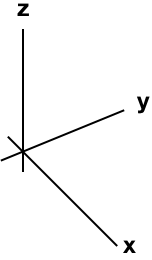
\includegraphics[scale=0.6]{img/C02axes.png}



\begin{tcolorbox}
The \textbf{scalar triple product} of vectors $\mb{u}$, $\mb{v}$, $\mb{w}$ is given by $\mb{u}\cdot(\mb{v}\times\mb{w})= \text{det}\left[\mb{u}\ \mb{v}\ \mb{w}\right]$.  The magnitude of the scalar triple product is the volume of the parallelepiped formed by the three vectors.

The \textbf{volume of a parallelepiped} with base given by the parallelogram formed by $\vec v$ and $\vec w$, and with the other sides formed by $\vec u$ has volume $\Vert \vec v \times \vec w\Vert\Vert (\vec u\Vert\vert\cos\theta\vert) =\vert \vec u\cdot(\vec v \times \vec w)\vert.$
\end{tcolorbox}

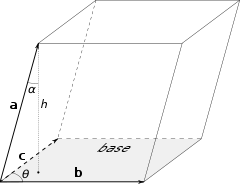
\includegraphics[]{img/C06scalartriple.png}

\url{https://en.wikipedia.org/wiki/Triple_product#/media/File:Parallelepiped_volume.svg}

\noindent\textbf{Cross product as a ``determinant''} \S 13.4

We have $\mb{u}\cdot(\mb{v}\times\mb{w}) = \text{det}[\mb{u}\ \mb{v}\ \mb{w}].$.

\begin{enumerate}
    \item This is $\text{det}[\mb{u}\ \mb{v}\ \mb{w}]=(u_1\mb{i}+u_2\mb{j}+u_3\mb{k})\cdot((v_2w_3-v_3w_2)\mb{i}+(v_3w_1-v_1w_3)\mb{j}+(v_1w_2-v_2w_1)\mb{k})$.
    \item Taking this dot product replaces the $\mb{i},\mb{j},\mb{k}$ in the second vector with the coefficients in the first vector: $\text{det}[\mb{u}\ \mb{v}\ \mb{w}]=(v_2w_3-v_3w_2)u_1+(v_3w_1-v_1w_3)u_2+(v_1w_2-v_2w_1)u_3$.
    \item Replacing $u_1,u_2,u_3$ with $\mb{i},\mb{j},\mb{k}$ in our determinant calculation will yield an expression for the cross product vector: $\mb{v}\times\mb{w} = \left\vert \begin{array}{c} \mb{i} \\ \mb{j} \\ \mb{k}\end{array} \ \mb{v}\ \mb{w}\right\vert = \left\vert \begin{array}{c} \mb{i}\ \mb{j}\ \mb{k}\\ \mb{v}^T \\ \mb{w}^T \end{array}\right\vert$.  This isn't a true determinant, but is a nice way to encode the formula for the cross product.
    \item We have $(v_2w_3-v_3w_2)\mb{i}+(v_3w_1-v_1w_3)\mb{j}+(v_1w_2-v_2w_1)\mb{k} = \left\vert\begin{array}{c c c} \mb{i} & \mb{j} & \mb{k} \\ v_1 & v_2 & v_3 \\ w_1 & w_2 & w_3 \end{array}\right\vert$
\end{enumerate}

\noindent\textbf{Example}

Find the cross product of $\mb{u} = \left(\begin{array}{c} 1 \\ 4 \\ 2\end{array}\right)$ and $\mb{v} = \left(\begin{array}{c} -2 \\ 0 \\ 1\end{array}\right)$.
\begin{align*}
\mb{u}\times\mb{v} &= \left\vert\begin{array}{c c c} \mb{i} & \mb{j} & \mb{k} \\ 1 & 4 & 2 \\ -2 & 0 & 1 \end{array}\right\vert = \mb{i}\left\vert\begin{array}{c c} 4 & 2 \\ 0 & 1 \end{array}\right\vert-\mb{j}\left\vert\begin{array}{c c} 1 & 2 \\ -2 & 1 \end{array}\right\vert+\mb{k}\left\vert\begin{array}{c c} 1 & 4 \\ -2 & 0 \end{array}\right\vert \\
&= \mb{i}(4)-\mb{j}(1-(-4))+\mb{k}(0-4(-2)) \\
&= 4\mb{i}-5\mb{j}+8\mb{k}
\end{align*}

Check in Matlab:
\begin{lstlisting}
cross([1 4 2],[-2 0 1])
\end{lstlisting}









\vspace{0.2cm}
\hrule
\vspace{0.2cm}





\noindent\textbf{Review questions}

\begin{questions}
\item True or False (discuss): There is only one point in the $yz$-plane that is distance $5$ from the point $(3,0,0)$.
\item Explain what is wrong with the statement: A contour diagram for $z = f(x,y)$ is a surface in $xyz$-space.
\item Explain what is wrong with the statement: The functions $f(x,y) = \sqrt{x^2+y^2}$ and $g(x,y) = x^2+y^2$ have the same contour diagram.

\item Sketch cross sections of the surface given by $x+y+z = 1$ with $y$ fixed.
\item Develop a method to find the intersection, if any, of the graphs of $f(x,y) = x^2+y^2$ and $g(x,y) = 1-x^2-y^2$.  The intersection of their graphs consists of $\{(x,y,z): z = f(x,y) = g(x,y)\}$.

\item Recall that linear functions can be written \[f(x,y) = mx + ny + d\] with the graph given by $z = mx + ny + d$.  They can also be written $f(x,y) = m (x-a) + n (y-b) + c$.

Consider the linear function $f(x,y) = 2(x-1) + (y-3) + 5$.  Find any three points in the graph of this function.

\item Find the linear function whose graph is the plane through the points $(4,0,0)$, $(0,3,0)$, $(0,0,2)$.

\item Let $f(x,y) = mx +ny + d$ where $m,n,d$ are constants and $n\neq 0$.  Show that the contour lines of $f$ are lines of slope $-\frac{m}{n}$.

\end{questions}

\end{document}